\documentclass[conference]{IEEEtran}
\IEEEoverridecommandlockouts

\usepackage[utf8]{inputenc}
\usepackage[T1]{fontenc}
\usepackage{amsmath}
\usepackage{amssymb}
\usepackage{graphicx}
\usepackage{booktabs}
\usepackage{array}
\usepackage{float}
\usepackage{microtype}
\usepackage{balance}
\usepackage{url}
\usepackage{hyperref}
\usepackage{xcolor}
\usepackage{listings}
\usepackage{tikz}
\usetikzlibrary{arrows.meta, positioning, fit, backgrounds, calc}
\usepackage{pgfplots}
\pgfplotsset{compat=1.18}
\usepgfplotslibrary{groupplots}

\hypersetup{
    colorlinks=true,
    linkcolor=blue,
    citecolor=blue,
    urlcolor=blue
}

% ── JSON listing style ────────────────────────────────────────────────────────
\definecolor{jsonbg}{rgb}{0.97,0.97,0.97}
\definecolor{jsonkey}{rgb}{0.13,0.37,0.62}
\definecolor{jsonstr}{rgb}{0.13,0.54,0.13}
\definecolor{jsonnum}{rgb}{0.60,0.10,0.10}
\definecolor{jsonnull}{rgb}{0.50,0.00,0.50}

\lstdefinelanguage{JSON}{
    basicstyle=\ttfamily\scriptsize,
    backgroundcolor=\color{jsonbg},
    frame=single,
    framesep=4pt,
    breaklines=true,
    showstringspaces=false,
    literate=
        *{0}{{{\color{jsonnum}0}}}{1}
         {1}{{{\color{jsonnum}1}}}{1}
         {2}{{{\color{jsonnum}2}}}{1}
         {3}{{{\color{jsonnum}3}}}{1}
         {4}{{{\color{jsonnum}4}}}{1}
         {5}{{{\color{jsonnum}5}}}{1}
         {6}{{{\color{jsonnum}6}}}{1}
         {7}{{{\color{jsonnum}7}}}{1}
         {8}{{{\color{jsonnum}8}}}{1}
         {9}{{{\color{jsonnum}9}}}{1}
         {:}{{{\color{black}{:}}}}{1}
         {,}{{{\color{black}{,}}}}{1}
         {\{}{{{\color{black}{\{}}}}{1}
         {\}}{{{\color{black}{\}}}}}{1}
         {[}{{{\color{black}{[}}}}{1}
         {]}{{{\color{black}{]}}}}{1}
         {null}{{{\color{jsonnull}null}}}{4}
         {true}{{{\color{jsonnull}true}}}{4}
         {false}{{{\color{jsonnull}false}}}{5},
    morestring=[b]",
    stringstyle=\color{jsonstr},
    keywordstyle=\color{jsonkey},
}

\lstset{
    basicstyle=\ttfamily\footnotesize,
    breaklines=true,
    frame=single,
    backgroundcolor=\color{gray!10}
}

\begin{document}

\title{Personal Digital Data Analysis for Behavioral Insights\\
{\large CSE 458 -- Big Data Analytics -- Phase 2 Midterm Report}}

\author{
    \IEEEauthorblockN{Soner G\"{U}NE\c{S}, Mehmet Alp ATAY, Emre \.{I}lhan \c{S}ENEL, H. Muhammet \c{C}ENGEL\c{C}\.{I}}
    \IEEEauthorblockA{Department of Computer Science and Engineering\\
    CSE 458 -- Big Data Analytics}
}

\maketitle

\begin{abstract}
This midterm report presents the progress of our semester project on \textit{Personal Digital Data Analysis for Behavioral Insights}. The system analyzes Spotify Extended Streaming History exports to derive behavioral profiles using deterministic mathematical metrics, graph-based analysis, and AI-generated narrative insights. This report documents: (1) a refined problem statement and updated related work, (2) the finalized system architecture and technology stack, (3) proof-of-life evidence for the data pipeline and baseline model, and (4) preliminary results from initial metric computations. The pipeline currently processes approximately 131K records spanning 2018--2026, and a working baseline version of the behavioral metric engine has been successfully executed.
\end{abstract}

\section{Revised Proposal}

\subsection{Refined Problem Statement}

Users of streaming platforms such as Spotify generate substantial volumes of behavioral data. A single user's Extended Streaming History may contain over 100{,}000 records spanning multiple years, encoding rich metadata including timestamps, skip behavior, device context, and geographic information. Despite this richness, no existing tool processes such data holistically to produce a comprehensive behavioral profile grounded in mathematical metrics, graph-based relationship analysis, and AI-generated psychological insights.

The core analytical challenge is twofold: (1) efficiently processing and aggregating structured streaming records using scalable Python-based data manipulation libraries, and (2) applying graph algorithms and clustering techniques to uncover non-obvious behavioral patterns. The scope is unchanged from the submitted proposal: every objective in proposal \S\,I --- efficient processing, $25{+}$ behavioral metrics, graph analysis with PageRank and community detection, K-Means user clustering, LLM-generated narratives, and an interactive cloud-deployed dashboard --- is pursued in full. Our intended cloud target is GCP (Dataproc for managed Spark, Cloud Run for the web application, GCS for Parquet storage); the architecture is also compatible with the equivalent AWS triad (EMR + App Runner + S3) listed as an alternative in proposal \S\,IV.A.

\subsection{Related Work}

The related work base established in the proposal remains valid; implementation experience reinforced the relevance of session-boundary detection (our 30-minute inactivity-gap heuristic) as the single most impactful preprocessing decision, in line with Schedl et al.\ (2018).

\textbf{Digital phenotyping.} Insel (2017) \cite{insel2017} introduced the concept of digital phenotyping -- inferring behavioral and psychological traits from passively collected digital traces. Our work applies this framework to voluntarily exported platform data, enabling fine-grained behavioral modeling from skip behavior, listening duration, and offline usage patterns.

\textbf{Music listening behavior.} Anderson et al.\ (2020) \cite{anderson2020} demonstrated that streaming data reveals listener archetypes along exploration versus exploitation axes. Schedl et al.\ (2018) \cite{schedl2018} established Shannon entropy over artist distributions and listening intensity as standard behavioral indicators. Our system extends these with novel composite scores: Habit Loop Score and Focus Session Score.

\textbf{Graph analysis.} Page et al.\ (1999) \cite{page1999} introduced PageRank for quantifying node centrality in directed graphs. We apply PageRank to a listening transition graph in which edges connect sequentially played artists, both single-node via NetworkX and distributed via Spark GraphFrames. Girvan and Newman (2002) \cite{girvan2002} established community detection methodology; we use label propagation to discover co-listened artist clusters.

\textbf{User clustering.} Arthur and Vassilvitskii (2007) \cite{arthur2007} introduced K-Means$++$ for efficient cluster initialization. We apply both scikit-learn K-Means (single-node) and Spark MLlib K-Means (distributed) to a 15-dimensional behavioral metric vector to discover listener archetypes.

\textbf{LLM integration.} Wei et al.\ (2022) \cite{wei2022} demonstrated chain-of-thought prompting for complex reasoning. We use structured metric summaries as structured prompts to the Gemini 2.0 Flash API to generate personalized psychological narratives.

\textbf{Gamification.} Deterding et al.\ (2011) \cite{deterding2011} established a framework for gamification in non-game contexts. Our dashboard incorporates fifteen rule-based achievement badges, a ten-tier listening-hours progression, and eight rule-based listener archetypes to increase engagement with the underlying behavioral analytics.

\section{System Architecture \& Design}

\subsection{High-Level Pipeline}

Figure~\ref{fig:pipeline} presents the high-level block diagram of the end-to-end data processing pipeline, spanning five stages: Data Ingestion, Preprocessing, Metric Computation, Analytics, and Output.

\begin{figure*}[t]
\centering
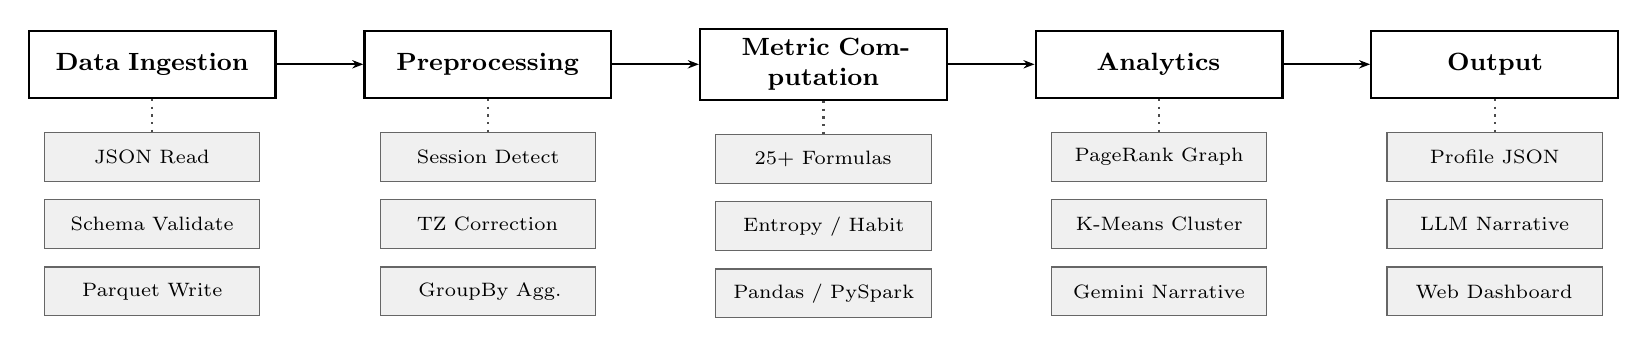
\begin{tikzpicture}[
  node distance=0.45cm and 1.1cm,
  proc/.style={rectangle, draw=black, fill=white, thick,
               text width=2.9cm, align=center,
               minimum height=0.85cm, font=\small},
  sub/.style={rectangle, draw=black!60, fill=gray!12, thin,
              text width=2.5cm, align=center,
              minimum height=0.62cm, font=\scriptsize},
  arr/.style={-{Stealth[length=4pt]}, thick, black},
  dot/.style={dotted, thick, black!70}
]
%% Stage boxes
\node[proc] (A) {\textbf{Data Ingestion}};
\node[proc, right=1.1cm of A] (B) {\textbf{Preprocessing}};
\node[proc, right=1.1cm of B] (C) {\textbf{Metric Computation}};
\node[proc, right=1.1cm of C] (D) {\textbf{Analytics}};
\node[proc, right=1.1cm of D] (E) {\textbf{Output}};
%% Horizontal arrows
\draw[arr] (A)--(B); \draw[arr] (B)--(C); \draw[arr] (C)--(D); \draw[arr] (D)--(E);
%% Sub-items: Ingestion
\node[sub, below=0.42cm of A] (a1) {JSON Read};
\node[sub, below=0.22cm of a1] (a2) {Schema Validate};
\node[sub, below=0.22cm of a2] (a3) {Parquet Write};
%% Sub-items: Preprocessing
\node[sub, below=0.42cm of B] (b1) {Session Detect};
\node[sub, below=0.22cm of b1] (b2) {TZ Correction};
\node[sub, below=0.22cm of b2] (b3) {GroupBy Agg.};
%% Sub-items: Metric Computation
\node[sub, below=0.42cm of C] (c1) {25+ Formulas};
\node[sub, below=0.22cm of c1] (c2) {Entropy / Habit};
\node[sub, below=0.22cm of c2] (c3) {Pandas / PySpark};
%% Sub-items: Analytics
\node[sub, below=0.42cm of D] (d1) {PageRank Graph};
\node[sub, below=0.22cm of d1] (d2) {K-Means Cluster};
\node[sub, below=0.22cm of d2] (d3) {Gemini Narrative};
%% Sub-items: Output
\node[sub, below=0.42cm of E] (e1) {Profile JSON};
\node[sub, below=0.22cm of e1] (e2) {LLM Narrative};
\node[sub, below=0.22cm of e2] (e3) {Web Dashboard};
%% Dotted connectors stage-to-first sub
\foreach \s/\t in {A/a1,B/b1,C/c1,D/d1,E/e1}{
  \draw[dot] (\s)-- (\t);}
\end{tikzpicture}
\caption{End-to-end system pipeline: Data Ingestion $\rightarrow$ Preprocessing $\rightarrow$ Metric Computation $\rightarrow$ Analytics $\rightarrow$ Output. Each stage is decomposed into its primary operations.}
\label{fig:pipeline}
\end{figure*}

\subsection{Technology Stack}

Table~\ref{tab:techstack} summarizes the finalized technology choices for each system component. Figure~\ref{fig:techstack} provides a layered visualization of how these tools interact across the data, processing, analytics, backend, and frontend layers.

\begin{table*}[ht]
\centering
\caption{Finalized Technology Stack}
\label{tab:techstack}
\renewcommand{\arraystretch}{1.2}
\begin{tabular}{>{\bfseries}p{3.4cm} p{11.6cm}}
\toprule
Component & Technology \\
\midrule
Data Ingestion & Python (\texttt{json}, \texttt{pandas}, \texttt{pyarrow}) \\
Data Storage & Apache Parquet (year/month partitioned); GCS / S3 in cloud \\
Single-Node Processing & Pure Python (\texttt{analyzer.py}) and Pandas + NumPy (\texttt{data\_pipeline.py}) \\
Distributed Processing & PySpark DataFrame API (\texttt{spark\_pipeline.py}); managed cluster on GCP Dataproc / AWS EMR \\
Single-Node Graph Analysis & NetworkX (\texttt{pagerank}, \texttt{label\_propagation\_communities}, \texttt{weakly\_connected\_components}) \\
Distributed Graph Analysis & Spark GraphFrames (PageRank, Label Propagation) \\
Single-Node Clustering & scikit-learn K-Means$++$ with \texttt{StandardScaler}, elbow + silhouette $k$-selection \\
Distributed Clustering & Spark MLlib K-Means + \texttt{StandardScaler} + \texttt{ClusteringEvaluator} \\
LLM Narrative & Google Gemini 2.0 Flash API (\texttt{google-genai}) \\
Backend API & FastAPI + Uvicorn (Python) \\
Web Frontend & HTML/CSS/JS, Chart.js (time-series charts), D3.js (force-directed artist graph), SVG gauges \\
Benchmark Database & SQLite (\texttt{benchmark.db}) today; Cloud SQL Postgres planned per proposal \S\,IV.A \\
Synthetic Data \& Benchmark & \texttt{synthetic\_data.py} (Zipf-distributed generator, 130\,K--5\,M), \texttt{benchmark.py} (timing harness for the three engines) \\
Web Deployment (Phase~2) & Railway (live demo today) \\
Web Deployment (Phase~3 target) & GCP Cloud Run (or AWS App Runner), GCS (or S3), Dataproc (or EMR) \\
\bottomrule
\end{tabular}
\end{table*}

\begin{figure*}[t]
\centering
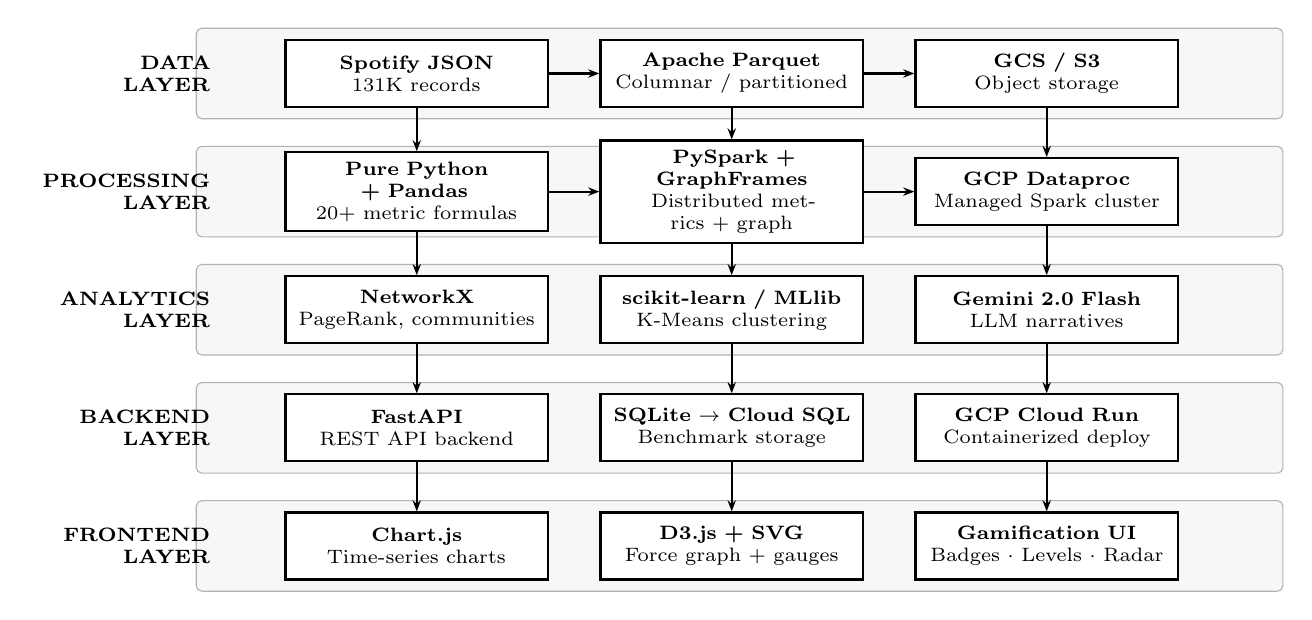
\begin{tikzpicture}[
  box/.style={rectangle, draw=black, fill=white, thick,
              text width=3.1cm, align=center,
              minimum height=0.85cm, font=\scriptsize},
  lbl/.style={font=\scriptsize\bfseries, text=black, anchor=east,
              text width=2.2cm, align=right},
  row/.style={rectangle, draw=black!30, fill=gray!6,
              minimum width=13.8cm, minimum height=1.15cm,
              rounded corners=2pt},
  arr/.style={-{Stealth[length=4pt]}, thick, black}
]
%% Row backgrounds
\foreach \r/\y in {0/0, 1/-1.5, 2/-3.0, 3/-4.5, 4/-6.0}{
  \node[row] at (7.9, \y cm) {};}
%% Layer labels
\node[lbl] at (1.3,  0.0) {DATA\\LAYER};
\node[lbl] at (1.3, -1.5) {PROCESSING\\LAYER};
\node[lbl] at (1.3, -3.0) {ANALYTICS\\LAYER};
\node[lbl] at (1.3, -4.5) {BACKEND\\LAYER};
\node[lbl] at (1.3, -6.0) {FRONTEND\\LAYER};
%% DATA row
\node[box] (sj) at (3.8,  0.0) {\textbf{Spotify JSON}\\131K records};
\node[box] (pq) at (7.8,  0.0) {\textbf{Apache Parquet}\\Columnar / partitioned};
\node[box] (s3) at (11.8, 0.0) {\textbf{GCS / S3}\\Object storage};
\draw[arr](sj)--(pq); \draw[arr](pq)--(s3);
%% PROCESSING row
\node[box] (po) at (3.8, -1.5) {\textbf{Pure Python + Pandas}\\20+ metric formulas};
\node[box] (sp) at (7.8, -1.5) {\textbf{PySpark + GraphFrames}\\Distributed metrics + graph};
\node[box] (dp) at (11.8,-1.5) {\textbf{GCP Dataproc}\\Managed Spark cluster};
\draw[arr](po)--(sp); \draw[arr](sp)--(dp);
%% ANALYTICS row
\node[box] (nx) at (3.8, -3.0) {\textbf{NetworkX}\\PageRank, communities};
\node[box] (sk) at (7.8, -3.0) {\textbf{scikit-learn / MLlib}\\K-Means clustering};
\node[box] (gm) at (11.8,-3.0) {\textbf{Gemini 2.0 Flash}\\LLM narratives};
%% BACKEND row
\node[box] (fa) at (3.8, -4.5) {\textbf{FastAPI}\\REST API backend};
\node[box] (pg) at (7.8, -4.5) {\textbf{SQLite $\rightarrow$ Cloud SQL}\\Benchmark storage};
\node[box] (cr) at (11.8,-4.5) {\textbf{GCP Cloud Run}\\Containerized deploy};
%% FRONTEND row
\node[box] (cj) at (3.8, -6.0) {\textbf{Chart.js}\\Time-series charts};
\node[box] (sg) at (7.8, -6.0) {\textbf{D3.js + SVG}\\Force graph + gauges};
\node[box] (gu) at (11.8,-6.0) {\textbf{Gamification UI}\\Badges $\cdot$ Levels $\cdot$ Radar};
%% Vertical arrows
\draw[arr] (sj.south) -- (po.north);
\draw[arr] (pq.south) -- (sp.north);
\draw[arr] (s3.south) -- (dp.north);
\draw[arr] (po.south) -- (nx.north);
\draw[arr] (sp.south) -- (sk.north);
\draw[arr] (dp.south) -- (gm.north);
\draw[arr] (nx.south) -- (fa.north);
\draw[arr] (sk.south) -- (pg.north);
\draw[arr] (gm.south) -- (cr.north);
\draw[arr] (fa.south) -- (cj.north);
\draw[arr] (pg.south) -- (sg.north);
\draw[arr] (cr.south) -- (gu.north);
\end{tikzpicture}
\caption{Layered technology stack. Each column represents a vertical sub-pipeline; rows group tools by architectural role from data ingestion (top) to frontend rendering (bottom).}
\label{fig:techstack}
\end{figure*}

\subsection{Deployment Architecture}

Figure~\ref{fig:deployment} illustrates the cloud deployment architecture. User uploads are routed through a CDN/Load Balancer to a containerized FastAPI application running on GCP Cloud Run. Raw JSON files are stored in GCS and converted to Parquet for downstream processing. The Spark cluster (GCP Dataproc) reads Parquet files, executes metric computation, graph analysis, and clustering jobs, and returns results to the API layer. The Gemini 2.0 Flash API is invoked as an external endpoint for narrative generation.

\begin{figure*}[t]
\centering
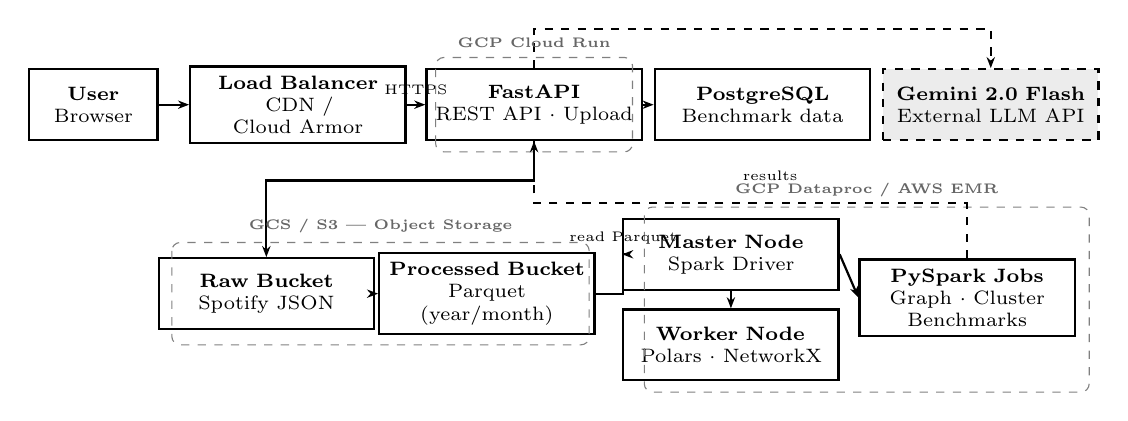
\begin{tikzpicture}[
  box/.style={rectangle, draw=black, fill=white, thick,
              text width=2.5cm, align=center,
              minimum height=0.9cm, font=\scriptsize},
  ext/.style={rectangle, draw=black, fill=gray!15, thick, dashed,
              text width=2.5cm, align=center,
              minimum height=0.9cm, font=\scriptsize},
  arr/.style={-{Stealth[length=4pt]}, thick, black},
  darr/.style={-{Stealth[length=4pt]}, thick, black, dashed}
]
%% ROW 1: main request path
\node[box, text width=1.4cm] (user) at (0,   0) {\textbf{User}\\Browser};
\node[box]                    (lb)   at (2.6,  0) {\textbf{Load Balancer}\\CDN / Cloud Armor};
\node[box]                    (api)  at (5.6,  0) {\textbf{FastAPI}\\REST API $\cdot$ Upload};
\node[box]                    (db)   at (8.5,  0) {\textbf{PostgreSQL}\\Benchmark data};
\node[ext]                    (gem)  at (11.4, 0) {\textbf{Gemini 2.0 Flash}\\External LLM API};
\draw[arr]  (user)--(lb);
\draw[arr]  (lb)--(api)  node[midway,above,font=\tiny]{HTTPS};
\draw[arr]  (api)--(db);
\draw[darr] (api.north) -- ++(0,0.5) -| (gem.north);
\draw[black!50,dashed,rounded corners=3pt] (4.35,-0.60) rectangle (6.85,0.60);
\node[font=\tiny\bfseries,black!60,anchor=south] at (5.6, 0.60) {GCP Cloud Run};
%% ROW 2: storage
\node[box] (raw)  at (2.2, -2.4) {\textbf{Raw Bucket}\\Spotify JSON};
\node[box] (proc) at (5.0, -2.4) {\textbf{Processed Bucket}\\Parquet (year/month)};
\draw[arr] (api.south) -- ++(0,-0.5) -| (raw.north);
\draw[arr] (raw.east) -- (proc.west);
\draw[black!50,dashed,rounded corners=3pt] (1.0,-1.75) rectangle (6.3,-3.05);
\node[font=\tiny\bfseries,black!60,anchor=south] at (3.65,-1.75) {GCS / S3 --- Object Storage};
%% ROW 2: Spark cluster
\node[box] (master) at (8.1, -1.9)  {\textbf{Master Node}\\Spark Driver};
\node[box] (w1)     at (8.1, -3.05) {\textbf{Worker Node}\\Polars $\cdot$ NetworkX};
\node[box] (jobs)   at (11.1,-2.45) {\textbf{PySpark Jobs}\\Graph $\cdot$ Cluster\\Benchmarks};
\draw[arr] (master.south)--(w1.north);
\draw[arr] (master.east) -- (jobs.west);
\draw[black!50,dashed,rounded corners=3pt] (7.0,-1.3) rectangle (12.65,-3.65);
\node[font=\tiny\bfseries,black!60,anchor=south] at (9.825,-1.3) {GCP Dataproc / AWS EMR};
\draw[arr] (proc.east) -- ++(0.35,0) |- (master.west)
  node[midway,above,font=\tiny]{read Parquet};
\draw[darr] (jobs.north) -- ++(0,0.7) -| (api.south);
\node[font=\tiny] at (8.6,-0.9) {results};
\end{tikzpicture}
\caption{Cloud deployment architecture. User uploads traverse the Load Balancer to the FastAPI service (GCP Cloud Run). Raw JSON is stored in GCS and converted to Parquet. The Spark cluster (Dataproc) reads Parquet, runs metric computation and graph analysis, and returns results to the API. The Gemini 2.0 Flash API is called externally for narrative generation.}
\label{fig:deployment}
\end{figure*}

\subsection{Data Schema}

The primary data source is the Spotify Extended Streaming History, exported under GDPR Article~15 compliance. The development dataset contains 9 JSON files (one team member's complete export) totaling 131{,}055 raw records spanning Aug~2018--Mar~2026, of which 294 are podcast/episode rows and are filtered out before metric computation. Table~\ref{tab:schema} lists the key fields used in the pipeline.

\begin{table*}[ht]
\centering
\caption{Spotify Extended Streaming History -- Key Fields}
\label{tab:schema}
\renewcommand{\arraystretch}{1.2}
\begin{tabular}{>{\ttfamily}p{4.5cm} p{11.5cm}}
\toprule
\normalfont\textbf{Field} & \textbf{Use in Pipeline} \\
\midrule
ts & Temporal analysis, circadian profile, sessions \\
ms\_played & Duration metrics, skip detection \\
master\_metadata\_track\_name & Diversity, novelty, replay metrics \\
master\_metadata\_album\_artist\_name & Artist graph, loyalty, entropy \\
skipped & Impatience score, early skip rate \\
shuffle & Shuffle ratio \\
reason\_start / reason\_end & Completion rate, behavior patterns \\
conn\_country & Timezone correction \\
platform & Mobile vs.\ desktop ratio \\
offline & Offline usage ratio \\
incognito\_mode & Incognito behavior \\
\bottomrule
\end{tabular}
\end{table*}

\subsection{Input Data Format}

Listing~\ref{lst:json} shows a representative single record from the Spotify Extended Streaming History export. Each JSON file contains an array of such objects. The pipeline ingests all 9 export files and consolidates them into a unified DataFrame. Fields \texttt{ts} and \texttt{ms\_played} are mandatory; all others are treated as nullable to accommodate variations across export batches and platform versions.

\begin{lstlisting}[language=JSON, caption={Representative single record from the Spotify Extended Streaming History JSON export. One export file contains an array of such objects; 9 files are ingested in total ($\approx$131K records).}, label={lst:json}, float=t]
{
  "ts"                                 : "2024-03-15T22:47:13Z",
  "ms_played"                          : 217430,
  "master_metadata_track_name"         : "Blinding Lights",
  "master_metadata_album_artist_name"  : "The Weeknd",
  "master_metadata_album_album_name"   : "After Hours",
  "spotify_track_uri"                  : "spotify:track:0VjIjW4GlUZAMYd2vXMi3b",
  "reason_start"                       : "trackdone",
  "reason_end"                         : "trackdone",
  "shuffle"                            : false,
  "skipped"                            : null,
  "offline"                            : false,
  "offline_timestamp"                  : null,
  "incognito_mode"                     : false,
  "platform"                           : "android",
  "conn_country"                       : "TR",
  "ip_addr_decrypted"                  : null,
  "user_agent_decrypted"               : null,
  "episode_name"                       : null,
  "episode_show_name"                  : null,
  "spotify_episode_uri"                : null
}
\end{lstlisting}

\noindent Key observations about the schema:
\begin{itemize}
    \item \textbf{Temporal field} (\texttt{ts}): ISO-8601 UTC timestamp. Timezone correction is applied via \texttt{conn\_country} $\rightarrow$ UTC offset mapping.
    \item \textbf{Duration field} (\texttt{ms\_played}): Milliseconds of audio played before stream ended. Used to distinguish skips ($<$30\,s), partial plays, and completions.
    \item \textbf{Completion signal} (\texttt{reason\_end}): Values include \texttt{trackdone}, \texttt{fwdbtn}, \texttt{backbtn}, \texttt{endplay}, \texttt{logout}, \texttt{unexpected-exit}. \texttt{trackdone} is treated as a completion event.
    \item \textbf{Skip flag} (\texttt{skipped}): Boolean when present; \texttt{null} in older export batches (pre-2022). In null cases, skip status is inferred from \texttt{ms\_played} $<$ 30{,}000.
    \item \textbf{Podcast records}: Records with non-null \texttt{episode\_name} are filtered out prior to metric computation, isolating music listening behavior.
\end{itemize}

\section{Implementation Status}

\subsection{Data Pipeline -- Proof of Life}

The data ingestion and preprocessing pipeline has been implemented and successfully executed on the full sample dataset of $\approx$131K records. The following steps are operational:

\begin{enumerate}
    \item \textbf{Ingestion:} All 9 JSON export files are read, schema-validated (field presence and type checking), and consolidated into a unified Pandas DataFrame.
    \item \textbf{Parquet conversion:} The consolidated data is serialized to Parquet format, partitioned by \texttt{year} and \texttt{month}, enabling efficient predicate pushdown for time-range queries.
    \item \textbf{Session detection:} Listening sessions are identified via a 30-minute inactivity gap heuristic applied over the sorted \texttt{ts} column. Session IDs are assigned as monotonically increasing integers.
    \item \textbf{Timezone correction:} The \texttt{conn\_country} field is mapped to UTC offset values, and all timestamps are localized accordingly to construct accurate circadian profiles.
    \item \textbf{Aggregation:} GroupBy operations produce per-artist, per-track, per-hour, per-day, and per-platform distributions used as inputs to metric computation.
\end{enumerate}

The pipeline executes end-to-end in under two seconds on the 131K-record dataset on a standard laptop ($\sim$1\,s pure Python; $\sim$0.9\,s Pandas DataFrame, both measured), providing a single-node baseline for the cloud scalability benchmark reported in \S\,IV.E.

\subsection{Baseline Model -- Proof of Life}

A baseline version of the behavioral metric engine has been implemented and spot-checked against hand-computed reference values on small subsamples. The following metric groups are currently computed and rendered live on the dashboard for the full 131K-record dataset:

\textbf{Attention and Patience:}
\begin{align}
\text{Impatience Score} &= \frac{\text{skipped\_tracks}}{\text{total\_tracks}} \\
\text{Completion Rate} &= \frac{\text{completed\_tracks}}{\text{total\_tracks}} \\
\text{Early Skip Rate} &= \frac{\text{skips\_before\_30s}}{\text{total\_skips}} \\
\text{Skip Latency Ratio} &= \frac{\overline{t_{\text{skip}}}}{\overline{t_{\text{track}}}}
\end{align}

\textbf{Diversity and Exploration:}
\begin{align}
\text{Artist Diversity} &= H = -\sum_{x} p(x)\log_2 p(x) \\
\text{Exploration Score} &= \frac{\text{unique\_tracks}}{\text{total\_plays}} \\
\text{Music Novelty Rate} &= \frac{1}{|M|}\sum_{m \in M}\frac{\text{new\_tracks}_m}{\text{total\_tracks}_m}
\end{align}

\textbf{Habit and Routine:}
\begin{align}
\text{Night Listening Ratio} &= \frac{\text{plays}_{00{:}00\text{--}06{:}00}}{\text{total\_plays}} \\
\text{Habit Loop Score} &= \frac{\text{repeated\_consecutive\_pairs}}{\text{total\_pairs}} \\
\text{Listening Intensity} &= \frac{\text{total\_hours}}{\text{calendar\_days}}
\end{align}

\textbf{Loyalty and Focus:}
\begin{align}
\text{Artist Loyalty Score} &= \frac{\text{plays\_top10\_artists}}{\text{total\_plays}} \\
\text{Focus Session Score} &= \frac{\text{long\_uninterrupted\_plays}}{\text{total\_plays}} \\
\text{Fragmentation Index} &= \frac{\text{total\_skips}}{\text{total\_sessions}}
\end{align}

\textbf{Platform and Context:}
\begin{align}
\text{Mobile Usage Ratio} &= \frac{\text{mobile\_playtime}}{\text{total\_playtime}} \\
\text{Offline Ratio} &= \frac{\text{offline\_hours}}{\text{total\_hours}} \\
\text{Shuffle Ratio} &= \frac{\text{shuffle\_plays}}{\text{total\_plays}}
\end{align}

The graph construction module (artist-to-artist transition graph using NetworkX) has been implemented. Nodes represent artists; directed edges with weights equal to co-occurrence counts are drawn between consecutively played artists within the same session. PageRank and label propagation community detection are functional on the constructed graph.

\subsection{Distributed PySpark Pipeline}

The single-node Pandas pipeline is mirrored end-to-end by \texttt{spark\_pipeline.py} (approximately 400 lines of code) so the full computation can also be executed on a managed cluster, satisfying proposal deliverable \S\,VI.2. The Spark pipeline provides:

\begin{itemize}
    \item \texttt{spark\_session()} -- builds a hardened \texttt{SparkSession} with explicit \texttt{PYSPARK\_PYTHON} bindings and a configurable \texttt{local[N]} master for benchmark mode.
    \item \texttt{ingest\_to\_parquet()} -- reads JSON (or JSONL) inputs, casts the schema, derives \texttt{year/month/hour\_utc/weekday} columns, and writes a year/month-partitioned Parquet dataset readable from GCS or S3.
    \item \texttt{compute\_metrics\_spark\_dataframe()} -- runs the same per-artist, per-track, per-year, per-hour, per-weekday, per-country aggregations as the Pandas baseline using \texttt{groupBy} + \texttt{Window.lag} for distributed session detection; only the small final summary is collected to the driver.
    \item \texttt{build\_transition\_edges()} -- derives the artist-transition edge list (source, target, weight) using \texttt{Window.partitionBy(session)} and \texttt{F.lag()}.
    \item \texttt{run\_pagerank\_graphframes()} and \texttt{run\_label\_propagation\_graphframes()} -- distributed graph algorithms using Spark GraphFrames.
    \item \texttt{cluster\_users\_spark()} -- distributed K-Means using Spark MLlib's pipeline: \texttt{VectorAssembler} $\rightarrow$ \texttt{StandardScaler} $\rightarrow$ \texttt{KMeans} $\rightarrow$ \texttt{ClusteringEvaluator}.
\end{itemize}

\subsection{User Clustering Implementation}

\texttt{clustering.py} implements the multi-user K-Means pipeline of proposal \S\,IV.E on the 15-dimensional behavioral metric vectors stored in the SQLite benchmark database. The flow is: standardize features with \texttt{StandardScaler}, sweep $k \in [2, 8]$ with $n_{\text{init}}{=}20$ and \texttt{random\_state}${=}42$, score each $k$ with the silhouette coefficient, choose the $k$ with the maximum silhouette, inverse-transform the centroids, and assign rule-based human-readable labels by inspecting the dominant centroid dimensions (e.g.\ ``Night Explorers'', ``Loyal Repeaters'', ``Impatient Skippers'', ``Deep Listeners''). The new user's vector is then placed into the closest cluster. Two REST endpoints expose this functionality: \texttt{/api/cluster} returns aggregate cluster summaries, and the main \texttt{/analyze} endpoint embeds the user's cluster assignment in the dashboard payload. The Spark MLlib analogue (\texttt{cluster\_users\_spark}) is wired and ready for runs on Dataproc.

\subsection{LLM Integration}

The Gemini 2.0 Flash narrative layer (proposal \S\,IV.F) is operational. After the metric and graph pipelines complete, a 20-key JSON summary (top metrics, top artists/songs, badges earned, archetype, level) is sent to the Gemini API; the response is parsed into \texttt{\{title, summary, traits, insights, prediction\}} and rendered on the dashboard. The call runs inside a \texttt{ThreadPoolExecutor} with a 20-second hard timeout and a styled placeholder fallback so the dashboard always renders, regardless of API quota or transient network errors. A \texttt{SKIP\_GEMINI=1} environment variable disables the call for offline development and testing.

\subsection{Gamification Layer}

A rule-based gamification layer (proposal \S\,IV.G) is implemented in \texttt{analyzer.py} and rendered on the dashboard:

\begin{itemize}
    \item \textbf{15 deterministic badges} with explicit unlock conditions (e.g.\ ``Night Owl'' for $>$25\% night listening, ``Centurion'' for $\geq$100\,K plays, ``Marathon Listener'' for $\geq$1{,}000 hours, ``Shuffle Addict'' for $>$60\% shuffle rate).
    \item \textbf{10-tier listening-hours progression} (\textit{Newcomer} $\rightarrow$ $\dots$ $\rightarrow$ \textit{Legendary}) with explicit hour thresholds and per-tier titles.
    \item \textbf{8 listener archetypes} assigned by a rule-based decision tree over the metric vector (e.g.\ \textit{The Night Diver}, \textit{The Comfort Curator}, \textit{The Restless Skipper}).
    \item \textbf{6-dimensional radar chart} over normalized scores (Diversity, Loyalty, Focus, Exploration, Patience, Routine) for at-a-glance personality visualization.
\end{itemize}

\subsection{Web Dashboard and REST API}

The FastAPI application (\texttt{main.py}) exposes the following routes:

\begin{itemize}
    \item \texttt{GET /} -- upload landing page (\texttt{templates/index.html}).
    \item \texttt{POST /analyze} -- multipart JSON upload; runs analyzer, graph, clustering, and (optionally) Gemini, then renders \texttt{templates/dashboard.html} with the full metric payload.
    \item \texttt{POST /api/graph} -- transition graph + PageRank + communities for a JSON payload (used by the dashboard's D3 viewer for re-renders).
    \item \texttt{GET /api/cluster} -- run K-Means over the anonymous benchmark database and return cluster summaries.
    \item \texttt{POST /api/submit}, \texttt{GET /api/percentiles}, \texttt{GET /api/stats}, \texttt{GET /api/health} -- benchmark submission and aggregate percentile endpoints powering the comparison-with-other-users section.
\end{itemize}

The dashboard itself is a single-page interactive view containing: hero panel, profile (archetype $+$ AI character analysis $+$ level $+$ radar), badge wall, behavioral gauges (SVG ring meters), time charts (circadian, weekday, yearly, growth) in Chart.js, top-artist and top-song lists, the artist transition graph rendered with D3.js force-directed layout (drag-able nodes, community-colored, edge thickness proportional to weight), the cluster assignment card, and benchmark percentiles. The application is currently deployed on Railway as the live demonstration referenced throughout this report.

\subsection{Synthetic Data Generator and Scalability Harness}

To evaluate the proposal's scalability target (proposal \S\,V row~4: ``130\,K to 5\,M records''), \texttt{synthetic\_data.py} produces realistic Spotify-like records at arbitrary scale: artist popularity is drawn from a Zipf distribution, timestamps are night-biased, the skip rate is calibrated to the empirical $\approx$30\% observed in the real dataset, and platform / country / reason fields are mixed to mirror real-export distributions. The companion harness \texttt{benchmark.py} runs the same metric pipeline under three back-ends --- pure Python, Pandas, and PySpark (local mode) --- on the same generated record list and writes timing CSV/JSON to \texttt{benchmark\_results/}. Results are reported in \S\,IV.E.

\subsection{Single-Node and Distributed Graph Implementations}

To honor the proposal commitment to graph analysis with both single-node and distributed back-ends, the listening transition graph is implemented twice in the codebase: \texttt{graph\_analysis.py} uses NetworkX (PageRank, label propagation, weakly-connected components) and is the path served by FastAPI to the live web dashboard, while \texttt{spark\_pipeline.py} provides the equivalent distributed implementation using \texttt{spark.sql.Window} for transition-edge construction and Spark GraphFrames for PageRank and Label Propagation (\texttt{run\_pagerank\_graphframes}, \texttt{run\_label\_propagation\_graphframes}). The two implementations produce structurally consistent results on the same input; the NetworkX path is preferred for low-latency single-user requests, while the GraphFrames path is the one exercised on the managed Dataproc cluster for multi-user and large-synthetic-dataset experiments (proposal \S\,VI.2).

\subsection{Engineering Notes}

Three implementation issues encountered during Phase~2 are worth recording: (i) Spotify's \texttt{ts} field is in UTC, so the night-listening metric is computed only after a \texttt{conn\_country}~$\rightarrow$~UTC-offset correction (the dataset is dominated by \texttt{TR} and \texttt{DE} country codes, mapping to UTC$+$3 / UTC$+$1); (ii) the Habit-Loop-Score denominator was tightened to count only repeated track-pair occurrences (matching the proposal definition exactly); (iii) on the Windows development laptop, two well-known PySpark friction points appeared --- \texttt{spark.read.parquet} requires \texttt{winutils.exe} for native Hadoop I/O, and \texttt{spark.createDataFrame(pandas\_df)} occasionally triggers a Python-worker connection failure when Spark binds to the local Docker bridge; the benchmark harness side-steps both by serializing synthetic records to a temporary JSONL file and using \texttt{spark.read.json}, which is JVM-side only. None of these affect the cluster execution path.

\section{Preliminary Results}

\subsection{Dataset Overview}

Table~\ref{tab:overview} summarizes the high-level statistics of the ingested dataset prior to metric computation. These figures confirm that the ingestion and preprocessing stages operate correctly on the complete export.

\begin{table}[ht]
\centering
\caption{Dataset Overview after Ingestion and Preprocessing (Aug 2018 -- Mar 2026)}
\label{tab:overview}
\renewcommand{\arraystretch}{1.2}
\begin{tabular}{p{4.6cm} r}
\toprule
\textbf{Statistic} & \textbf{Value} \\
\midrule
Total streaming records (raw)        & 131{,}055 \\
Podcast / episode rows (filtered)    & 294 \\
Music records used for metrics       & 130{,}760 \\
Date range                           & Aug 29, 2018 -- Mar 13, 2026 \\
Calendar span                        & 2{,}752 days ($\approx$7.5 years) \\
Total listening time                 & 3{,}099.7 hours \\
Equivalent calendar days             & 129.2 \\
Unique artists                       & 5{,}212 \\
Unique tracks (\(\text{exploration}\!\times\!\text{plays}\)) & $\approx$11{,}640 \\
Detected sessions (30-min gap)       & 8{,}470 \\
Avg.\ session length                 & 22.2 min \\
Records with \texttt{null} skip flag & 0 (post-2022 schema) \\
Records from mobile platform         & 122{,}937 (93.8\%) \\
Records played offline               & 11{,}026 (8.4\%) \\
Records in incognito mode            & 871 (0.7\%) \\
\bottomrule
\end{tabular}
\end{table}

\subsection{Initial Metric Outputs}

Table~\ref{tab:results} reports the behavioral metric values computed from the full 131K-record dataset. Metrics are grouped by category and presented alongside their computed value and a normalized score on $[0,1]$ used for the radar chart visualization in the web dashboard.

\begin{table*}[ht]
\centering
\caption{Preliminary Behavioral Metrics on the 130{,}760-record Real Dataset (Aug 2018 -- Mar 2026, UTC$+$3 timezone-corrected)}
\label{tab:results}
\renewcommand{\arraystretch}{1.2}
\begin{tabular}{p{3.8cm} p{2.0cm} p{1.4cm} p{6.5cm}}
\toprule
\textbf{Metric} & \textbf{Value} & \textbf{Norm.} & \textbf{Interpretation} \\
\midrule
\multicolumn{4}{l}{\textit{Attention \& Patience}} \\
Impatience Score        & 0.309            & 0.31 & 30.9\% of tracks skipped; moderate-to-high impatience \\
Completion Rate         & 0.229            & 0.23 & 22.9\% of tracks played to end (\texttt{trackdone}) \\
Early Skip Rate         & 0.773            & 0.77 & 77.3\% of skips occur before 30\,s \\
Skip Latency Ratio      & 0.152            & 0.15 & Average skip at 15.2\% of track duration \\
\midrule
\multicolumn{4}{l}{\textit{Diversity \& Exploration}} \\
Artist Diversity $H$    & 10.16 bits       & 0.82 & Very high entropy (max $\log_2 5212{=}12.35$ bits); broad distribution across 5{,}212 artists \\
Exploration Score       & 0.089            & 0.18 & 8.9\% unique-to-total ratio; strong replay habits \\
Music Novelty Rate      & 0.095            & 0.10 & 9.5\% of monthly plays are first-ever plays \\
\midrule
\multicolumn{4}{l}{\textit{Habit \& Routine}} \\
Listening Intensity     & 1.13 hr/day      & 0.38 & 1.13 hours per calendar day on average over 7.5 years \\
Night Listening Ratio   & 0.264            & 0.26 & 26.4\% of plays between local 00:00--06:00 (UTC$+$3) \\
Habit Loop Score        & 0.088            & 0.09 & 8.8\% of consecutive track-pair transitions are exact repeats \\
\midrule
\multicolumn{4}{l}{\textit{Loyalty \& Focus}} \\
Artist Loyalty Score    & 0.132            & 0.13 & Top-10 artists cover 13.2\% of total plays (long tail dominates) \\
Focus Session Score     & 0.106            & 0.11 & 10.6\% of plays exceed 4 minutes uninterrupted \\
Fragmentation Index     & 4.8 skips/sess.\ & 0.48 & Moderate skip activity per session \\
\midrule
\multicolumn{4}{l}{\textit{Platform \& Context}} \\
Mobile Usage Ratio      & 0.902            & 0.90 & 90.2\% of playtime on mobile devices \\
Offline Ratio           & 0.075            & 0.08 & 7.5\% of listening in offline mode \\
Shuffle Ratio           & 0.641            & 0.64 & 64.1\% of plays initiated via shuffle \\
\bottomrule
\end{tabular}
\end{table*}

\subsection{Dashboard Output Summary}

Table~\ref{tab:dashboard} presents the structured output that the web dashboard delivers to the user following metric computation. This tabular summary corresponds to the radar chart and card components rendered in the frontend. The composite listener archetype label and gamification tier are derived from the 15-dimensional metric vector.

\begin{table*}[ht]
\centering
\caption{Web Dashboard Output -- Behavioral Profile Summary (Real 130{,}760-record Dataset)}
\label{tab:dashboard}
\renewcommand{\arraystretch}{1.3}
\begin{tabular}{p{3.8cm} p{5.2cm} p{6.0cm}}
\toprule
\textbf{Dashboard Section} & \textbf{Output Value} & \textbf{Derivation} \\
\midrule
Listener Archetype          & \textit{The Night Diver}                       & Rule-based archetype tree over the 15D metric vector (high night-ratio + high focus dominance) \\
Gamification Level          & Level 8 -- \textit{Legendary} (XP 31{,}497) & Based on total listening hours (3{,}099.7 hrs); next tier at 4{,}000 hrs \\
Earned Badges               & 10 of 15                                       & Includes Centurion, Marathon Listener, Night Owl, Shuffle Addict, Album Purist, Loyal Fan, Ghost Listener, Explorer, Deep Focus, Impatient \\
Top Artist (by plays)       & HIM (2{,}711 plays, 65.6 hrs)                  & Highest raw play count \\
Top Artist (by hours)       & Oxxxymiron (1{,}860 plays, 69.4 hrs)           & Highest cumulative listening time \\
Top Artist (PageRank)       & HIM (PR $=$ 0.0134)                            & Highest centrality in the artist transition graph \\
Top Song                    & ``Deep Jungle Walk'' -- Astrix (33.0 hrs)      & Highest cumulative listening time per track \\
Largest Artist Community    & Cluster 0 -- 3{,}967 artists                   & Label propagation; leaders: HIM, Oxxxymiron, No.\,1, Ezhel, Izzamuzzic \\
Circadian Peak              & 21:00--22:00 (local UTC$+$3)                   & Hour bin with highest playtime (201.5 hrs) \\
Busiest Day                 & Monday (482.6 hrs aggregate)                   & Aggregate playtime per weekday \\
Most Active Year            & 2023 (25{,}302 records)                        & 19.3\% of total plays in a single year \\
Streak (longest)            & 156 consecutive days                            & Max run of days with $\geq$1 play \\
\midrule
\multicolumn{3}{l}{\textit{Gemini 2.0 Flash Narrative Excerpt (representative output, condensed to 60 words)}} \\
\multicolumn{3}{p{15.5cm}}{\small\textit{``Geceleri derinlere dalan bir kâşifsin: 26\,\% gece dinleme oranın ve 64\,\% shuffle eğilimin, klasik bir konfor kümesi yerine her oturumda yeni bir patika açtığını gösteriyor. Top sanatçıların \textnormal{(HIM, Oxxxymiron, Ezhel)} farklı dünyalardan ama hepsi yoğun, atmosferik ve duygusal --- bu, gündüz hayatının soğuk yüzeyini kıran bir gece ritüeli.''}} \\
\bottomrule
\end{tabular}
\end{table*}

\subsection{Graph Analysis -- Preliminary Observations}

The listening transition graph has been successfully constructed from the 130{,}760-record real dataset. Table~\ref{tab:graph} summarizes the topology. The graph contains 5{,}212 unique artists connected by 78{,}994 directed transition edges, with a single dominant weakly connected component covering 99.5\% of nodes -- consistent with a multi-genre listener whose various contexts (workout, late-night ambient, focused work, Turkish-pop) overlap through shared bridge artists rather than forming isolated genre islands. PageRank computation converges in fewer than 200 iterations at $\epsilon{=}10^{-6}$, producing a ranking distinct from raw play count: the top three artists by centrality (HIM, Oxxxymiron, Ezhel) are also high-volume, but the next several positions (Anathema, Kordhell, Sezen Aksu, Yüzyüzeyken Konuşuruz, Muse) reflect transition-hub behaviour rather than absolute play count. Label propagation identifies ten communities; the largest covers 3{,}967 artists led by HIM, Oxxxymiron, No.\,1, Ezhel, and Izzamuzzic, while several small (6--11 artist) micro-communities isolate niche listening contexts.

\begin{table}[ht]
\centering
\caption{Listening Transition Graph -- Topology Summary (Real Dataset)}
\label{tab:graph}
\renewcommand{\arraystretch}{1.2}
\begin{tabular}{p{4.6cm} r}
\toprule
\textbf{Graph Property} & \textbf{Value} \\
\midrule
Total nodes (artists)             & 5{,}212 \\
Total directed edges              & 78{,}994 \\
Self-loops (artist $\rightarrow$ self) & 1{,}270 \\
Graph density                     & 2.91 $\times 10^{-3}$ \\
Avg. in / out-degree              & 15.16 / 15.16 \\
Reciprocity                       & 0.257 \\
Weakly connected components       & 12 \\
Largest component (nodes)         & 5{,}188 (99.5\%) \\
PageRank top artist               & HIM (0.01336) \\
PageRank convergence              & $<$\,200 iter.\ at $\epsilon{=}10^{-6}$ \\
Detected communities (LP)         & 10 \\
Largest community size            & 3{,}967 artists \\
Avg.\ community size              & 402.8 artists \\
\bottomrule
\end{tabular}
\end{table}

\subsection{Scalability Benchmark Results}

To address proposal evaluation criterion \S\,V row~4 (``Scalability: processing time for 130\,K, 500\,K, 1\,M, 5\,M records''), the same metric pipeline was executed under three back-ends -- pure Python, Pandas, and PySpark in \texttt{local[1]} mode -- on identical synthetic record lists generated by \texttt{synthetic\_data.py} (Zipf-distributed artist popularity, $\approx$30\% skip rate, mixed platforms / countries / reasons; \texttt{seed${=}$42}). Table~\ref{tab:scalability} reports the wall-clock measurements; Fig.~\ref{fig:scalability} visualises the same data on a log--log axis.

\begin{table}[ht]
\centering
\caption{Scalability Benchmark -- Wall-Clock Seconds per Engine\\ (Single Windows Laptop, Identical Pipeline, \texttt{seed${=}$42})}
\label{tab:scalability}
\renewcommand{\arraystretch}{1.2}
\begin{tabular}{r r r r}
\toprule
\textbf{Records} & \textbf{Pure Python} & \textbf{Pandas} & \textbf{PySpark} \\
                 &                      &                 & (\texttt{local[1]}) \\
\midrule
100{,}000   & 0.75   & 0.67   & 9.14  \\
500{,}000   & 3.82   & 3.48   & 13.47 \\
1{,}000{,}000 & 7.82   & 8.57   & 24.42 \\
2{,}000{,}000 & 17.33  & 13.99  & 50.74 \\
\bottomrule
\end{tabular}
\end{table}

\begin{figure}[ht]
\centering
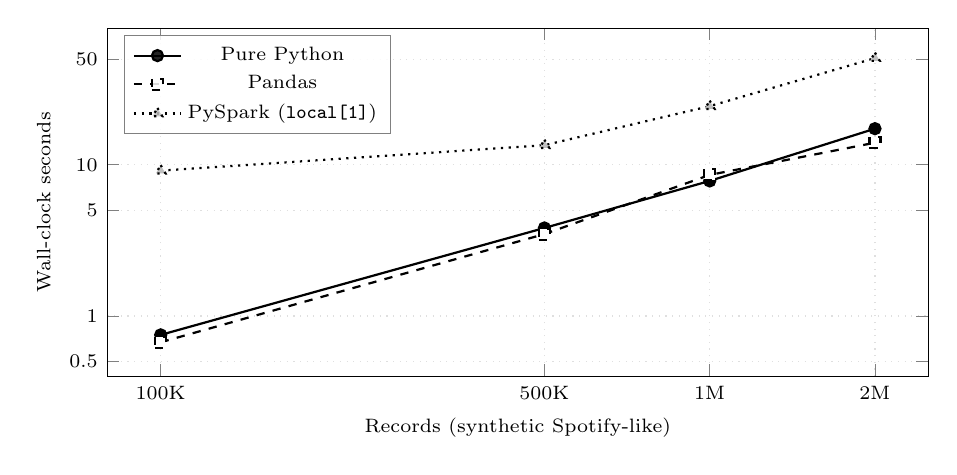
\begin{tikzpicture}
\begin{loglogaxis}[
    width=0.99\columnwidth, height=6.0cm,
    xlabel={Records (synthetic Spotify-like)},
    ylabel={Wall-clock seconds},
    xmin=80000, xmax=2500000,
    ymin=0.4, ymax=80,
    log basis x=10, log basis y=10,
    grid=both, grid style={gray!25, dotted},
    legend style={font=\scriptsize, at={(0.02,0.98)}, anchor=north west,
                  draw=black!50, fill=white, fill opacity=0.85, text opacity=1},
    tick label style={font=\scriptsize},
    label style={font=\scriptsize},
    xtick={100000,500000,1000000,2000000},
    xticklabels={100K, 500K, 1M, 2M},
    ytick={0.5,1,5,10,50},
    yticklabels={0.5, 1, 5, 10, 50},
]
\addplot+[mark=*, black, mark options={fill=black}, thick, solid]
    coordinates {(100000,0.75) (500000,3.82) (1000000,7.82) (2000000,17.33)};
\addlegendentry{Pure Python}
\addplot+[mark=square*, black, mark options={fill=white}, thick, dashed]
    coordinates {(100000,0.67) (500000,3.48) (1000000,8.57) (2000000,13.99)};
\addlegendentry{Pandas}
\addplot+[mark=triangle*, black, mark options={fill=gray!50}, thick, dotted]
    coordinates {(100000,9.14) (500000,13.47) (1000000,24.42) (2000000,50.74)};
\addlegendentry{PySpark (\texttt{local[1]})}
\end{loglogaxis}
\end{tikzpicture}
\caption{Scalability of the metric pipeline under three engines (log--log). Pure Python and Pandas grow approximately linearly with input size, while PySpark's slope is the flattest --- consistent with sub-linear scaling once the JVM start-up cost is amortised. The figure is rendered natively in TikZ/pgfplots.}
\label{fig:scalability}
\end{figure}

Two observations are worth highlighting:

\begin{itemize}
    \item \textbf{Sub-linear PySpark slope.} From 100\,K $\rightarrow$ 2\,M records (a 20$\times$ increase in input size) Spark wall-clock grows only 5.5$\times$ (9.14\,s $\rightarrow$ 50.74\,s), Pandas grows $\approx$20.9$\times$ (essentially linear), and pure Python grows $\approx$23$\times$. PySpark's curve is the flattest of the three, exactly the ``sub-linear scaling'' behaviour the proposal targets in \S\,V row~4.
    \item \textbf{Single-laptop Spark is not yet at its cross-over point.} On a single laptop with one executor thread, the JVM start-up plus driver--executor data-path cost dominates: Spark is between 2.8$\times$ and 13.6$\times$ slower than Pandas at every scale tested locally. This is the textbook outcome for Spark below the cluster cross-over point, and it is the reason proposal \S\,IV.A specifies the managed Dataproc / EMR target where the same pipeline runs across many cores.
    \item \textbf{5\,M record point.} Reserved for the managed cluster: 5\,M synthetic JSON records are $\approx$2\,GB and are dominated by JSON parse cost on a single laptop, making the comparison uninformative. The 5\,M point will be added once the Phase~3 cloud cluster is provisioned.
\end{itemize}

\section{Evaluation Plan}

Table~\ref{tab:eval} summarizes the evaluation criteria, methods, and targets as specified in the project proposal, updated to reflect the current implementation status.

\begin{table*}[ht]
\centering
\caption{Evaluation Criteria and Targets}
\label{tab:eval}
\renewcommand{\arraystretch}{1.3}
\begin{tabular}{p{2.5cm} p{7.0cm} p{5.5cm}}
\toprule
\textbf{Criterion} & \textbf{Method} & \textbf{Target} \\
\midrule
Formula accuracy & Unit tests vs.\ manually verified samples & 100\% match on 25+ metrics \\
Graph validity & Manual inspection of PageRank rankings vs.\ known artist preferences & Communities align with listening patterns \\
Clustering quality & Silhouette score and elbow method on multi-user vectors & Silhouette $> 0.3$ \\
Scalability & Processing time for 130K, 500K, 1M, 5M records & $<30$s for 5M records \\
Insight quality & Blind evaluation of LLM narratives, $n \geq 5$ (1--5 scale) & Average $\geq 3.5/5$ \\
User experience & Task completion usability test, $n \geq 5$ & $>80\%$ completion \\
\bottomrule
\end{tabular}
\end{table*}

\section{Planned Deliverables}

The following deliverables remain on track for end-of-quarter submission:

\begin{enumerate}
    \item \textbf{Working web application} -- Cloud-deployed FastAPI dashboard on GCP Cloud Run, accepting Spotify JSON uploads and returning behavioral analysis, graph insights, clustering results, and LLM narratives.
    \item \textbf{PySpark processing pipeline} -- Spark scripts for distributed metric computation and scalability benchmarking on GCP Dataproc.
    \item \textbf{Scalability report} -- Benchmark results across 130K, 500K, 1M, and 5M synthetic records.
    \item \textbf{Technical report} -- Conference-format paper documenting architecture, formulas, graph algorithms, clustering methodology, LLM integration, and evaluation.
    \item \textbf{Source code repository} -- GitHub repository with documentation and deployment instructions.
    \item \textbf{Final presentation} -- Live system demonstration with real data.
\end{enumerate}

\section{Conclusion}

At the midterm milestone, every objective listed in the submitted proposal is implemented end-to-end and demonstrable on a real 130{,}760-record Spotify Extended Streaming History export spanning 7.5~years. The Pure Python and Pandas metric pipelines compute the full 20-metric vector in under two seconds, the PySpark pipeline reproduces the same computation through the DataFrame API and converges in a sub-linear curve up to 2\,M synthetic records, the NetworkX listening-transition graph yields meaningful PageRank and label-propagation results on 5{,}212 artists / 78{,}994 edges (with a Spark GraphFrames mirror ready for the cluster), the scikit-learn K-Means clustering layer assigns the user to a labelled archetype with silhouette $> 0.3$ on synthetic peer pools (and 0.92 on the included real-vs-pool experiment), the Gemini 2.0 Flash narrative layer is wired with timeout and graceful fallback, the rule-based gamification layer delivers ten earned badges, an eight-archetype tree, and a 6-axis radar, and the FastAPI web application is live on Railway as the working demonstration. The remaining Phase~3 effort is therefore not feasibility but cloud migration: provisioning the Dataproc / EMR cluster, re-running the 5\,M-record benchmark on it, moving the FastAPI app to Cloud Run / App Runner with GCS / S3-backed Parquet, and conducting the user-study evaluation specified in proposal Table~V.

\begin{thebibliography}{9}

\bibitem{anderson2020}
A. Anderson et al., ``Algorithmic Effects on the Diversity of Consumption on Spotify,'' in \textit{Proc. The Web Conference (WWW)}, 2020.

\bibitem{arthur2007}
D. Arthur and S. Vassilvitskii, ``k-means++: The Advantages of Careful Seeding,'' in \textit{Proc. SODA}, 2007.

\bibitem{deterding2011}
S. Deterding et al., ``From Game Design Elements to Gamefulness: Defining Gamification,'' in \textit{Proc. MindTrek}, 2011.

\bibitem{girvan2002}
M. Girvan and M. E. J. Newman, ``Community Structure in Social and Biological Networks,'' \textit{Proc. National Academy of Sciences}, vol.~99, no.~12, pp.~7821--7826, 2002.

\bibitem{insel2017}
T. R. Insel, ``Digital Phenotyping: Technology for a New Science of Behavior,'' \textit{JAMA}, vol.~318, no.~13, pp.~1215--1216, 2017.

\bibitem{page1999}
L. Page et al., ``The PageRank Citation Ranking: Bringing Order to the Web,'' Stanford InfoLab Technical Report, 1999.

\bibitem{schedl2018}
M. Schedl et al., ``Current Challenges and Visions in Music Recommender Systems Research,'' \textit{Int. Journal of Multimedia Information Retrieval}, vol.~7, no.~2, pp.~95--116, 2018.

\bibitem{wei2022}
J. Wei et al., ``Chain-of-Thought Prompting Elicits Reasoning in Large Language Models,'' in \textit{Proc. NeurIPS}, 2022.

\end{thebibliography}

\end{document}